\documentclass[tikz,border=10pt]{standalone}
\usetikzlibrary{positioning,arrows.meta,fit,backgrounds}

\definecolor{coreindigo}{HTML}{3F51B5}
\definecolor{ifgreen}{HTML}{4CAF50}
\definecolor{fsgray}{HTML}{757575}
\definecolor{localgray}{HTML}{9E9E9E}
\definecolor{syncgreen}{HTML}{4CAF50}

\begin{document}
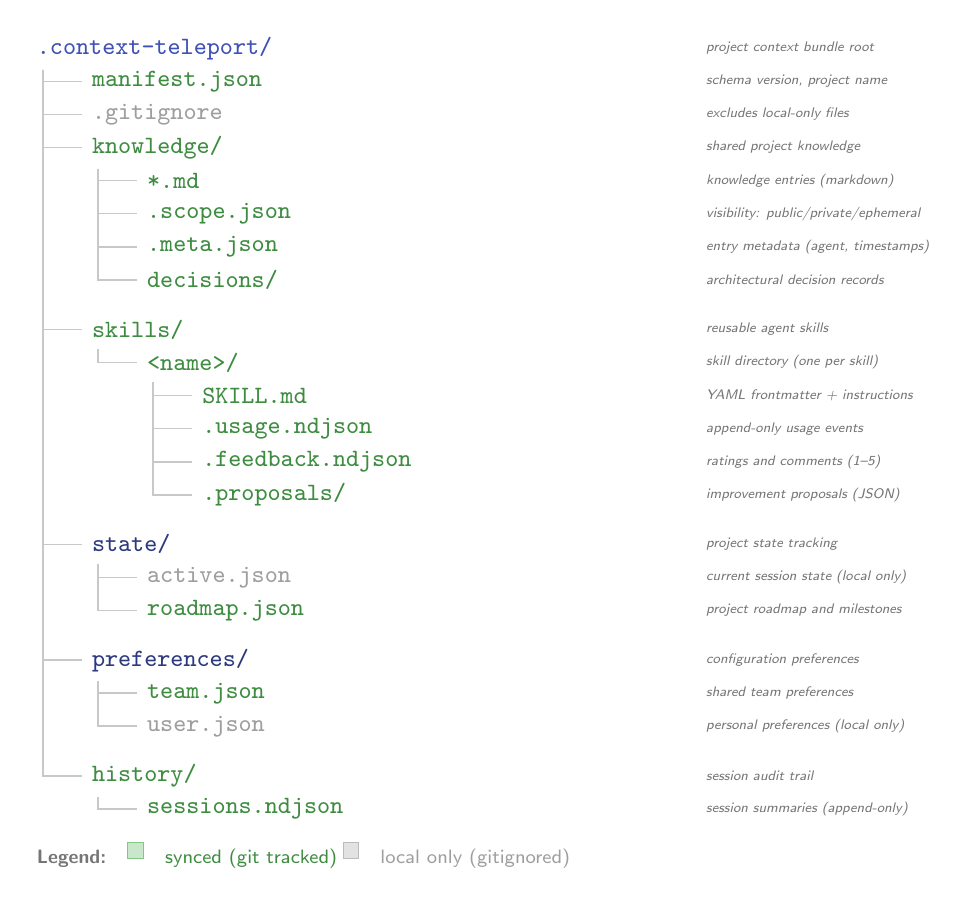
\begin{tikzpicture}[
    every node/.style={font=\sffamily},
    treenode/.style={
        anchor=west, font=\sffamily\small
    },
    synced/.style={treenode, text=syncgreen!80!black},
    local/.style={treenode, text=localgray},
    mixed/.style={treenode, text=coreindigo!70!black},
    annot/.style={font=\sffamily\tiny\itshape, text=fsgray, anchor=west},
    treeline/.style={color=fsgray!40, line width=0.6pt},
]

% Spacing constants
\def\indent{0.7cm}
\def\dindent{1.4cm}
\def\tindent{2.1cm}
\def\vgap{0.42cm}
\def\annotoff{8.5cm}

% Root
\node[treenode, font=\sffamily\small\bfseries, text=coreindigo] (root) at (0,0)
    {\texttt{.context-teleport/}};
\node[annot] at (\annotoff, 0) {project context bundle root};

% --- Level 1 children ---
% manifest.json
\node[synced] (manifest) at (\indent, -\vgap) {\texttt{manifest.json}};
\node[annot] at (\annotoff, -\vgap) {schema version, project name};

% .gitignore
\node[local] (gitign) at (\indent, -2*\vgap) {\texttt{.gitignore}};
\node[annot] at (\annotoff, -2*\vgap) {excludes local-only files};

% knowledge/
\node[synced, font=\sffamily\small\bfseries] (know) at (\indent, -3*\vgap) {\texttt{knowledge/}};
\node[annot] at (\annotoff, -3*\vgap) {shared project knowledge};

% knowledge children
\node[synced] (knowmd) at (\dindent, -4*\vgap) {\texttt{*.md}};
\node[annot] at (\annotoff, -4*\vgap) {knowledge entries (markdown)};

\node[synced] (knowscope) at (\dindent, -5*\vgap) {\texttt{.scope.json}};
\node[annot] at (\annotoff, -5*\vgap) {visibility: public/private/ephemeral};

\node[synced] (knowmeta) at (\dindent, -6*\vgap) {\texttt{.meta.json}};
\node[annot] at (\annotoff, -6*\vgap) {entry metadata (agent, timestamps)};

\node[synced, font=\sffamily\small\bfseries] (decisions) at (\dindent, -7*\vgap) {\texttt{decisions/}};
\node[annot] at (\annotoff, -7*\vgap) {architectural decision records};

% skills/
\node[synced, font=\sffamily\small\bfseries] (skills) at (\indent, -8.5*\vgap) {\texttt{skills/}};
\node[annot] at (\annotoff, -8.5*\vgap) {reusable agent skills};

% skills children
\node[synced, font=\sffamily\small\bfseries] (skillname) at (\dindent, -9.5*\vgap) {\texttt{<name>/}};
\node[annot] at (\annotoff, -9.5*\vgap) {skill directory (one per skill)};

\node[synced] (skillmd) at (\tindent, -10.5*\vgap) {\texttt{SKILL.md}};
\node[annot] at (\annotoff, -10.5*\vgap) {YAML frontmatter + instructions};

\node[synced] (skillusage) at (\tindent, -11.5*\vgap) {\texttt{.usage.ndjson}};
\node[annot] at (\annotoff, -11.5*\vgap) {append-only usage events};

\node[synced] (skillfb) at (\tindent, -12.5*\vgap) {\texttt{.feedback.ndjson}};
\node[annot] at (\annotoff, -12.5*\vgap) {ratings and comments (1--5)};

\node[synced, font=\sffamily\small\bfseries] (proposals) at (\tindent, -13.5*\vgap) {\texttt{.proposals/}};
\node[annot] at (\annotoff, -13.5*\vgap) {improvement proposals (JSON)};

% state/
\node[mixed, font=\sffamily\small\bfseries] (state) at (\indent, -15*\vgap) {\texttt{state/}};
\node[annot] at (\annotoff, -15*\vgap) {project state tracking};

\node[local] (active) at (\dindent, -16*\vgap) {\texttt{active.json}};
\node[annot] at (\annotoff, -16*\vgap) {current session state (local only)};

\node[synced] (roadmap) at (\dindent, -17*\vgap) {\texttt{roadmap.json}};
\node[annot] at (\annotoff, -17*\vgap) {project roadmap and milestones};

% preferences/
\node[mixed, font=\sffamily\small\bfseries] (prefs) at (\indent, -18.5*\vgap) {\texttt{preferences/}};
\node[annot] at (\annotoff, -18.5*\vgap) {configuration preferences};

\node[synced] (team) at (\dindent, -19.5*\vgap) {\texttt{team.json}};
\node[annot] at (\annotoff, -19.5*\vgap) {shared team preferences};

\node[local] (user) at (\dindent, -20.5*\vgap) {\texttt{user.json}};
\node[annot] at (\annotoff, -20.5*\vgap) {personal preferences (local only)};

% history/
\node[synced, font=\sffamily\small\bfseries] (hist) at (\indent, -22*\vgap) {\texttt{history/}};
\node[annot] at (\annotoff, -22*\vgap) {session audit trail};

\node[synced] (sessions) at (\dindent, -23*\vgap) {\texttt{sessions.ndjson}};
\node[annot] at (\annotoff, -23*\vgap) {session summaries (append-only)};

% ============================
% Tree lines (parent -> child connections)
% ============================

% Helper: vertical line from parent down, then horizontal to child
% Root to level-1 children
\foreach \child/\yidx in {manifest/1, gitign/2, know/3, skills/8.5, state/15, prefs/18.5, hist/22} {
    \draw[treeline] ([xshift=0.2cm]root.south west) |- (\child.west);
}

% knowledge/ to its children
\foreach \child in {knowmd, knowscope, knowmeta, decisions} {
    \draw[treeline] ([xshift=0.2cm]know.south west) |- (\child.west);
}

% skills/ to <name>/
\draw[treeline] ([xshift=0.2cm]skills.south west) |- (skillname.west);

% <name>/ to its children
\foreach \child in {skillmd, skillusage, skillfb, proposals} {
    \draw[treeline] ([xshift=0.2cm]skillname.south west) |- (\child.west);
}

% state/ to its children
\foreach \child in {active, roadmap} {
    \draw[treeline] ([xshift=0.2cm]state.south west) |- (\child.west);
}

% preferences/ to its children
\foreach \child in {team, user} {
    \draw[treeline] ([xshift=0.2cm]prefs.south west) |- (\child.west);
}

% history/ to its children
\draw[treeline] ([xshift=0.2cm]hist.south west) |- (sessions.west);

% ============================
% Legend
% ============================
\node[font=\sffamily\scriptsize\bfseries, text=fsgray, anchor=west] (legend) at (0, -24.5*\vgap) {Legend:};
\node[synced, font=\sffamily\scriptsize, right=0.5cm of legend] (lsync) {synced (git tracked)};
\node[local, font=\sffamily\scriptsize, right=0.3cm of lsync] (llocal) {local only (gitignored)};

% Small colored squares for legend
\fill[syncgreen!30] ([xshift=-0.35cm]lsync.west) rectangle ++(0.2,0.2);
\draw[syncgreen!70, line width=0.4pt] ([xshift=-0.35cm]lsync.west) rectangle ++(0.2,0.2);
\fill[localgray!30] ([xshift=-0.35cm]llocal.west) rectangle ++(0.2,0.2);
\draw[localgray!70, line width=0.4pt] ([xshift=-0.35cm]llocal.west) rectangle ++(0.2,0.2);

\end{tikzpicture}
\end{document}
